\documentclass[xcolor=dvipsnames,10pt,aspectratio=169]{beamer}
%\documentclass[xcolor=dvipsnames,10pt]{beamer}
\usepackage{etex}
\usepackage{pgf,pgfarrows,pgfnodes,pgfautomata,pgfheaps,pgfshade}
\usepackage[absolute,overlay]{textpos} 
%\usepackage{algorithm}
\usepackage{amsmath,amssymb}
\usepackage[utf8]{inputenc} 
\usepackage{colortbl}
\usepackage{graphicx} 
\usepackage[brazil]{babel}
\usepackage{tabularx} 
\usepackage{multirow}
\usepackage{booktabs}
\usepackage{listings}
%\usepackage{multimedia}
\usepackage{animate}
\usepackage{xcolor}
\usepackage{array}
\usepackage{longtable}
\usepackage{makecell}
\usepackage{caption}
\usetheme{Madrid} 
\usepackage{amsmath}
\usepackage{movie15}
\usepackage{tikz}
\usetikzlibrary{shapes.geometric,arrows,shadows}

%Definição dos layers.
\pgfdeclarelayer{background}
\pgfdeclarelayer{foreground}
\pgfsetlayers{background,main,foreground}



\lstset{ %
%	backgroundcolor=\color{white},   % choose the background color; you must add \usepackage{color} or \usepackage{xcolor}
%	basicstyle=\footnotesize,        % the size of the fonts that are used for the code
	basicstyle=\scriptsize,        % the size of the fonts that are used for the code
	breakatwhitespace=false,         % sets if automatic breaks should only happen at whitespace
	breaklines=true,                 % sets automatic line breaking
	captionpos=t,                    % sets the caption-position to bottom
	commentstyle=\color{mygreen},    % comment style
	deletekeywords={...},            % if you want to delete keywords from the given language
	escapeinside={\%*}{*)},          % if you want to add LaTeX within your code
	extendedchars=true,              % lets you use non-ASCII characters; for 8-bits encodings only, does not work with UTF-8
%	frame=single,                    % adds a frame around the code
	keepspaces=true,                 % keeps spaces in text, useful for keeping indentation of code (possibly needs columns=flexible)
	keywordstyle=\color{blue},       % keyword style
%	language=make,                 % the language of the code
	morekeywords={*,...},            % if you want to add more keywords to the set
%	numbers=left,                    % where to put the line-numbers; possible values are (none, left, right)
%	numbersep=5pt,                   % how far the line-numbers are from the code
	numberstyle=\tiny\color{mygray}, % the style that is used for the line-numbers
	rulecolor=\color{black},         % if not set, the frame-color may be changed on line-breaks within not-black text (e.g. comments (green here))
	showspaces=false,                % show spaces everywhere adding particular underscores; it overrides 'showstringspaces'
	showstringspaces=false,          % underline spaces within strings only
	showtabs=false,                  % show tabs within strings adding particular underscores
	stepnumber=2,                    % the step between two line-numbers. If it's 1, each line will be numbered
}

\definecolor{mygreen}{rgb}{0,0.6,0}
\definecolor{mygray}{rgb}{0.5,0.5,0.5}
\definecolor{mymauve}{rgb}{0.58,0,0.82}

\usecolortheme{beaver}
\newcommand{\ul}{\underline}
\setbeamertemplate{footline}{\scriptsize{\vspace*{0.3cm}\hspace*{15cm}\insertframenumber\,/\,\inserttotalframenumber}}
\setbeamertemplate{caption}[numbered]
\setbeamerfont{caption}{size=\fontsize{8}{5}}

\setbeamercolor{block title}{	bg=Sepia , fg = White}
\setbeamercolor{block body}{bg=Brown!15, fg=Sepia }
\setbeamercolor{item projected}{bg=Sepia, fg=White}
\setbeamercolor{number projected}{bg = Black}

%declara as imagens usadas no layout do slide
\pgfdeclareimage[height=0.8cm]{mflab}{figuras_presentation_template/logo_mflab_transparente.png}
\pgfdeclareimage[height=1.0cm]{logoufu}{figuras_presentation_template/logo_ufu.jpg}
\pgfdeclareimage[height=1.0cm]{petro}{figuras_presentation_template/petrobras_2.png}

%posiciona o logotipo do MFLab
\setlength{\TPHorizModule}{1mm}
\setlength{\TPVertModule}{1mm}
\newcommand{\placelogomflab} 
{ 
	\begin{textblock}{13}(150.0,0.0)
		\pgfuseimage{mflab} 
	\end{textblock} 
	
% 	\begin{textblock}{13}(128.0,1.0)
% 		\pgfuseimage{logoufu} 
% 	\end{textblock} 
	
	\begin{textblock}{13}(150.0,70.0)
		\pgfuseimage{petro} 
	\end{textblock} 
}
%posiciona o logotipo do MFLab
\setlength{\TPHorizModule}{1mm}
\setlength{\TPVertModule}{1mm}
\newcommand{\placelogo} 
{ 
	\begin{textblock}{13}(150.0,0.0)
		\pgfuseimage{mflab} 
	\end{textblock} 
	
% 	\begin{textblock}{13}(128.0,1.0)
% 		\pgfuseimage{logoufu} 
% 	\end{textblock} 
	
	\begin{textblock}{13}(0.0,80.0)
		\pgfuseimage{petro} 
	\end{textblock} 
}

% \setlength{\TPHorizModule}{1mm}
% \setlength{\TPVertModule}{1mm}
% \newcommand{\placelogomflab_titulo} 
% { 
% 	\begin{textblock}{13}(150.0,0.0)
% 		\pgfuseimage{mflab} 
% 	\end{textblock} 
% 	
% 	\begin{textblock}{13}(0.0,0.0)
% 		\pgfuseimage{lmest} 
% 	\end{textblock} 
% 	
% % 	\begin{textblock}{13}(128.0,1.0)
% % 		\pgfuseimage{logoufu} 
% % 	\end{textblock} 
% 	
% 	\begin{textblock}{13}(75.0,80.0)
% 		\pgfuseimage{petro} 
% 	\end{textblock} 
% }



%insere o logotipo da ufu em todos os slides
% \logo{
\includegraphics[height=0.8cm]{figuras/layout_slide/petrobras.png}}

\title{Iniciativa Rayleigh:Escoamentos em cavidade, uma análise bidimensional com implementação de MPI e OPENGL.}

\author{ Felipe J. O. Ribeiro \\ \and \\ Orientador: Prof. Dr. Aristeu da Silveira Neto}

%\date{\tiny{02 de dezembro de 2015}}
\date{\tiny{\today}}
% \newcolumntype{M}[1]{>{\raggedright\arraybackslash}b{#1}}
% \newcolumntype{N}{@{}m{0pt}@{}}	
% \newcolumntype{M}{>{\begin{minipage}[b]{3cm}\raggedright{}}c<{\end{minipage}\minrowheight}}
% \setlength\extrarowheight{5pt}
\newcolumntype{C}[1]{>{\centering\let\newline\\\arraybackslash\hspace{0pt}}m{#1}}


\begin{document}
	
	
	

	\begin{frame}\placelogomflab
		\frametitle 
		{ \vfill
			\centering
			{
			\small{Universidade Federal de Uberlândia}\\
%			\small{Programa de Pós-Graduação em Engenharia Mecânica}\\
			\small{Laboratório de Mecânica dos Fluidos}\\
			}
		}
		\maketitle
	\end{frame}




	
\section<presentation>*{Sumário}
	
	\begin{frame}
		\frametitle{Sumário}\placelogomflab 
		{\scriptsize \tableofcontents}
	\end{frame}





	\AtBeginSection[]
	{
	\begin{frame}<beamer>
		\frametitle{Sumário}\placelogomflab 
		{\scriptsize \tableofcontents[current,currentsection]}
	\end{frame}
	}
	\AtBeginSubsection[]
	{
	\begin{frame}<beamer>
		  \frametitle{Sumário}\placelogomflab 
		  {\scriptsize \tableofcontents[current,currentsubsection]}
	\end{frame}
	}





%%%%%%%%%%%%%%%%%%%%%%%%%%%%%%%%%%%%%%%%%%%%%%%%%%%%%%%%%%%%%%%%%%%%%%%%%%%%%%%%%%%%%%%%%%%%%%
\section{Introdução}
	
	\begin{frame}
		\frametitle{Objetivos}
					
		\centering
		O presente texto procura documentar o desenvolvimento deste trabalho de pesquisa com o máximo de detalhes nas metodologias possível. Dês dos desenvolvimentos matemáticos e teóricos aos andamentos nos aspectos técnicos e organizacionais.
		
		\vspace{0.5cm}
		
		\flushleft
		Os tópicos centrais deste estudo são:\\
		\quad $\bullet$ Desenvolvimento teórico e matemático do escoamento bidimensional em cavidade.\\
		\quad $\bullet$ Implementação de modelo de turbulência baseado na hipótese de Boussinesq. \\
		\quad $\bullet$ Desenvolvimento das conversões dos parâmetros do Poiseuille para a cavidade.\\
		\quad $\bullet$ Aperfeiçoamento dos protocolos de visualização de dados com OpenGL.\\
		\quad $\bullet$ Desenvolvimento das rotinas em MPI no domínio bidimensional.\\
		
	\end{frame}





	\begin{frame}
		\frametitle{Estrutura de arquivos}
		\begin{tabular}{c c}
			{
				\begin{minipage}[h!]{0.15\textwidth}
					\centering
					\small
					Neste projeto, dês do início, será dada uma atenção especial à organização dos documentos, de forma a simplificar o andamento das atividades de documentação e prosseguimento.
					\vspace{6cm}
				\end{minipage}
			}&{
				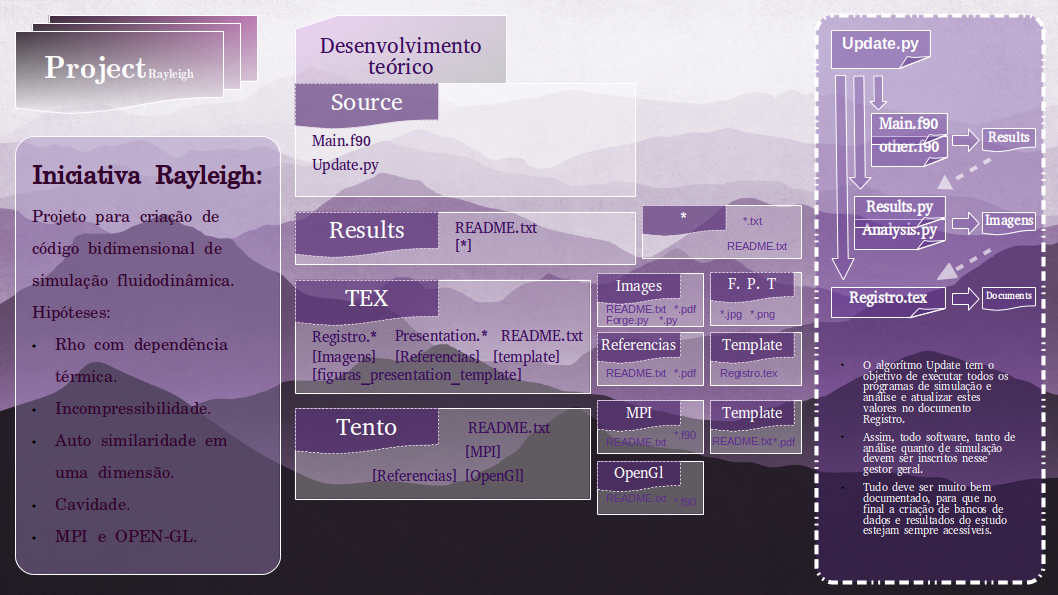
\includegraphics[trim={0.0cm 0.0cm 0.0cm 0.0cm},clip=true, scale = 0.435]{../../arquivos.pdf}
			}
		\end{tabular}

	\end{frame}





	\begin{frame}
		\frametitle{Documento "Registro.tex"}
		\begin{tabular}{c c}
			{
				\begin{minipage}[h!]{0.4\textwidth}
					\centering
					\small
					Por questões de adequações á formatação em textos científicos, além desta apresentação também serão registrados os andamentos nesse documento em inglês. Ele segue o template da ASME para textos científicos. Assim, pretende-se já desenvolver as rotinas de visualização dos resultados de acordo com estas convenções. De forma a facilitar a criação de documentos para submissão em artigos e tornando este processo mais ágil.
					\vspace{6cm}
				\end{minipage}
			}&{
				\includegraphics[page = 1,trim={0.0cm 12.0cm 0.0cm 0.0cm},clip=true, scale = 0.4]{registro.pdf}
			}	
		\end{tabular}
	
	\end{frame}





	\begin{frame}
		\frametitle{Levante bibliográfico}
		\begin{minipage}[h!]{0.33\textwidth}
			\begin{figure}
				\centering
				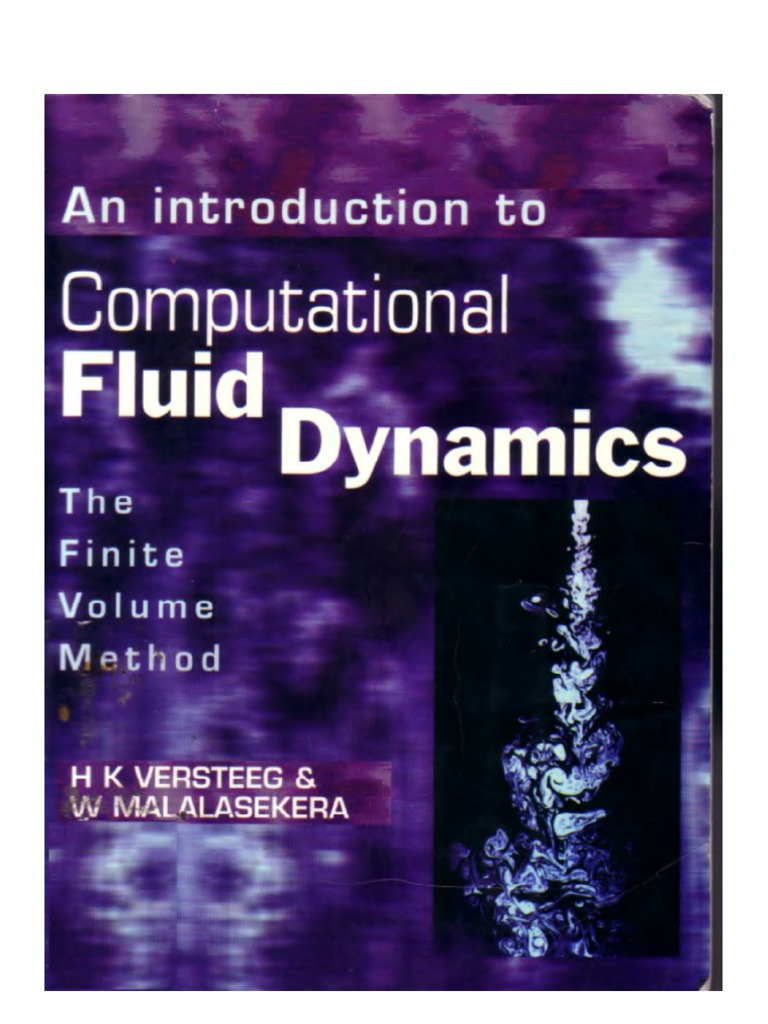
\includegraphics[page = 1,trim={0.0cm 0.0cm 0.0cm 0.0cm},clip=true, scale = 0.15]{Referencias/An_introduction_to_Computational}
				\caption{Possui as referencias aos métodos matemáticos e numéricos de modelagem e discretização da fluidodinâmica ao domínio bidimensional.}	
			\end{figure}
			\vspace{6cm}
		\end{minipage}
		\begin{minipage}[h!]{0.33\textwidth}
			\begin{figure}
				\centering
				
\includegraphics[page = 1,trim={0.0cm 0.0cm 0.0cm 0.0cm},clip=true, scale = 0.165]{Referencias/MPI_Guide_FORTRAN.png}\\	
				\caption{Um guia para se aprender a desenvolver em FORTRAN as rotinas em paralelo, com passagem de mensagem entre os processos.}
			\end{figure}
			\vspace{6cm}
		\end{minipage}
		\begin{minipage}[h!]{0.325\textwidth}
			\begin{figure}
				\centering
				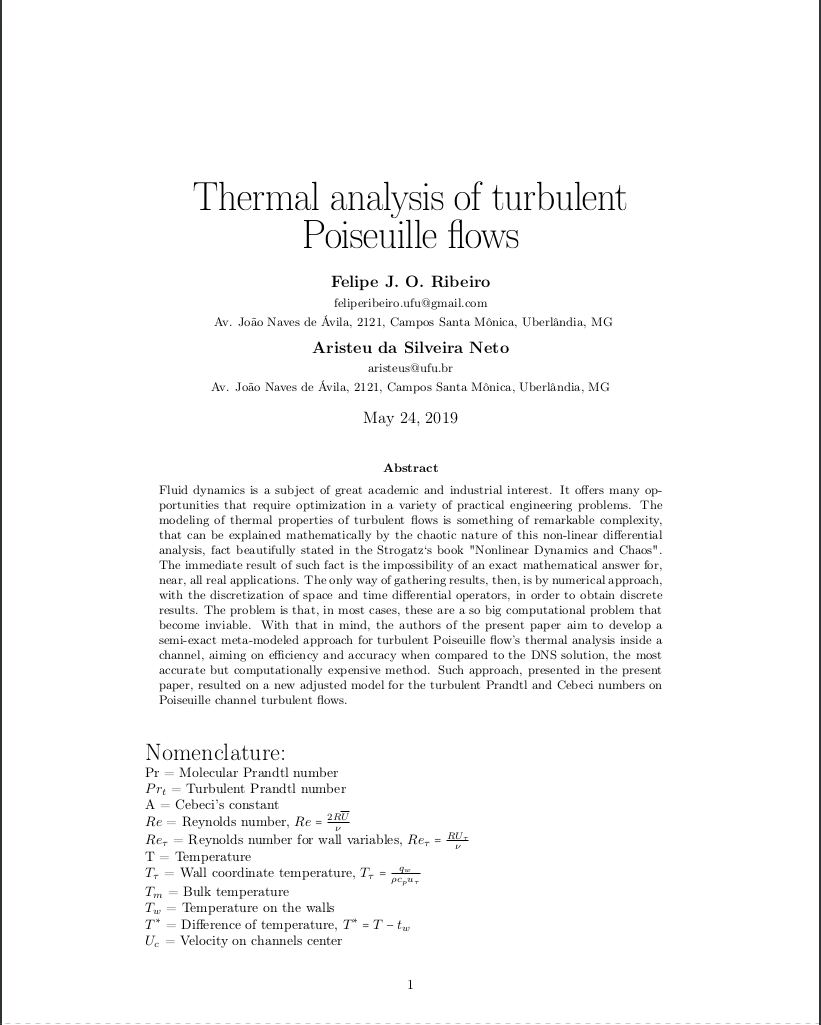
\includegraphics[page = 1,trim={1.0cm 1.0cm 1.0cm 0.0cm},clip=true, scale = 0.165]{Referencias/Projeto_cebeci}\\
				\caption{Artigo previamente publicado, para resgate dos ajustes paramétricos.}
			\end{figure}
			\vspace{6cm}
		\end{minipage}
	
	\end{frame}





	\begin{frame}
		\frametitle{Análise térmica bidimensional e tridimensional}
		$\bullet$ A advecção natural é um fenômeno de turbulência clássico. Ele apresenta muitos exemplos tanto industriais quanto práticos do dia a dia. 
		Para se simular tal fenômeno um domínio bi ou tridimensional é necessário (tridimensional se modelos de turbulência são implementados). Dessa forma torna-se uma extensão natural do trabalho desenvolvido até o momento. Apesar de lidar com mudanças de massa dos fluidos, ainda não se chega a se tratar de compressibilidade. Dessa forma, nesse trabalho espera-se:

		- Desenvolver modelos 2D e 3D representativos.

		- Implementar métodos de otimização conforme necessários, como mpi e opengl.

		- Desenvolver método de apresentação visual integrado ao fortran. 

		\begin{figure}[h!]
			\centering
			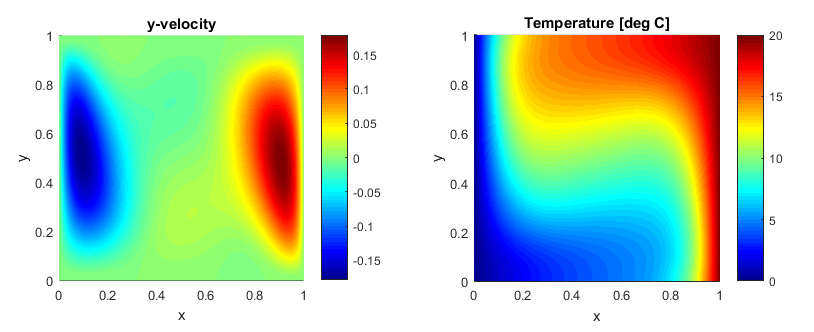
\includegraphics[trim = {1.7cm 2cm 0 1cm}, clip , angle=0, scale=0.50]{images/NaturalConvectionFromNet}
			\caption{Convecção natural.}
		\end{figure}

	\end{frame}
	
%%%%%%%%%%%%%%%%%%%%%%%%%%%%%%%%%%%%%%%%%%%%%%%%%%%%%%%%%%%%%%%%%%%%%%%%%%%%%%%%%%%%%%%%%%%%%%
\section{Estudos introdutórios}

	
	
	
	\begin{frame} 
		\frametitle{Domínio bidimensional com advecção imposta}
		\begin{minipage}[h!]{0.49\textwidth}
			$\bullet$ Converter código bidimensional antigo em MatLab para c++.\\
			$\bullet$ Desenvolver advecção, com velocidades em $x$ e $y$ impostas para todo o domínio.\\
			$\bullet$ Desenvolver biblioteca visual para este estudo com openGL.\\
			$\bullet$ Converter para o fortran os códigos.\\
			$\bullet$ Experimentar plataforma openGL com fortran.\\
			$\bullet$ Estudar acoplamento velocidade pressão.\\
		\end{minipage}
		\begin{minipage}[h!]{0.49\textwidth}
			\begin{figure}[h!]
				\centering
				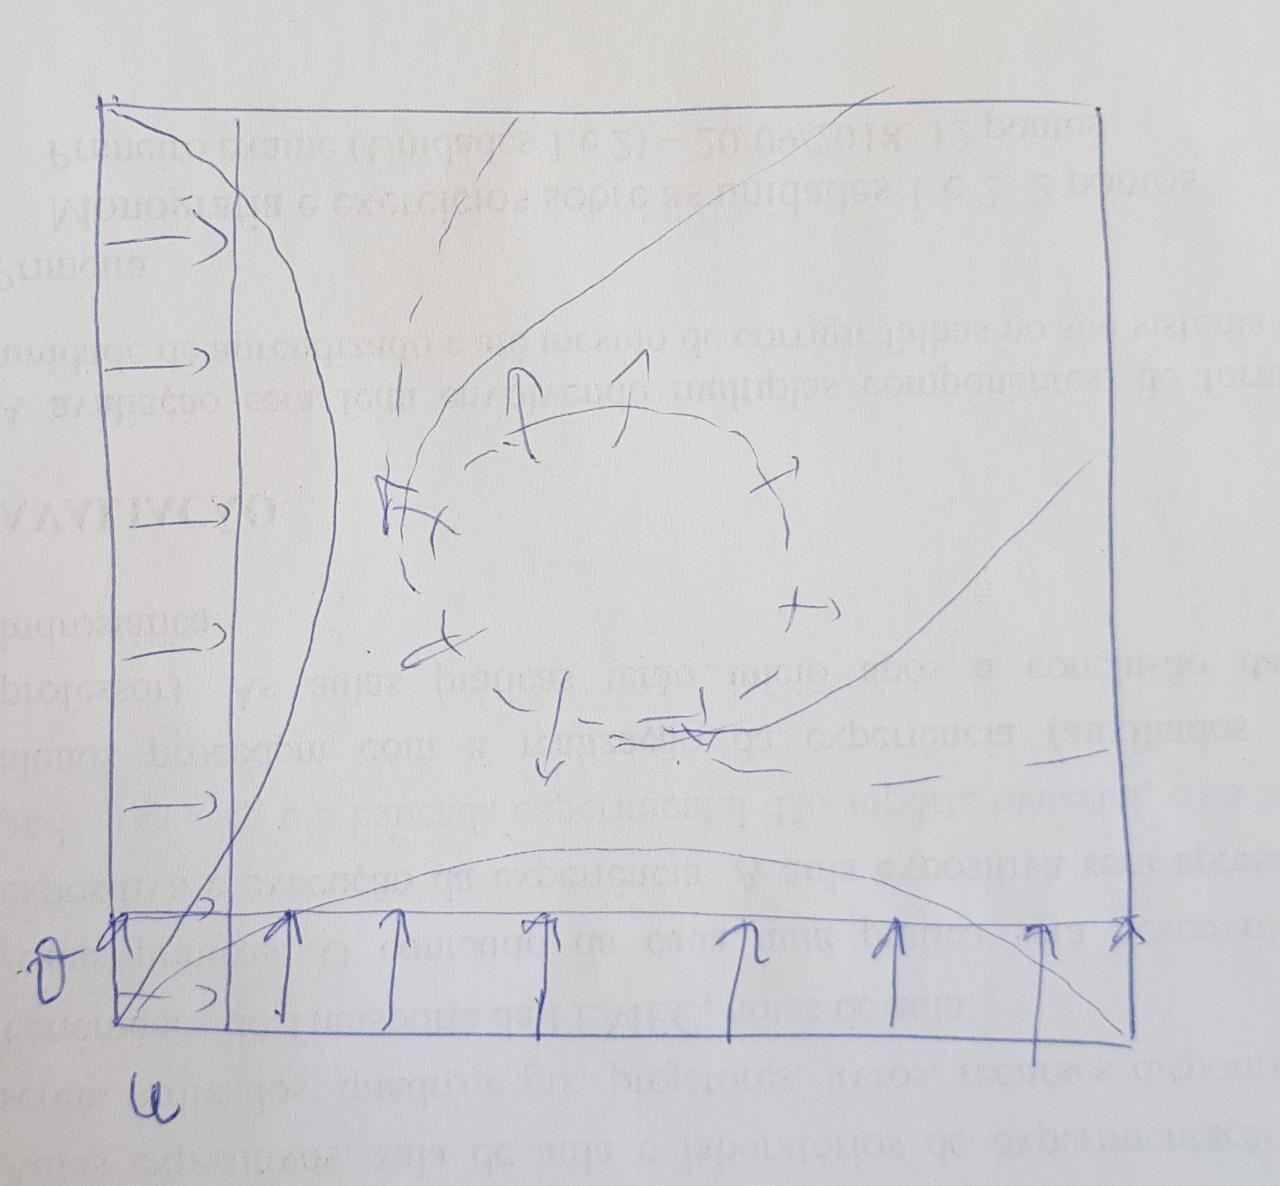
\includegraphics[trim = {0cm 1cm 0 1cm}, clip , angle=0, scale=0.15]{images/ImagemProfessor1}
				\caption{Esquema do professor.}
			\end{figure}
		\end{minipage}
	\end{frame}



	\begin{frame} 
		\frametitle{Modelo matemático diferencial}
		$\bullet$ A equação de balanço da energia térmica foi desenvolvida como base, com termos advectivos.\\
		$\bullet$ A dimensão $z$ foi ignorada, considerando-se auto similaridade neste eixo.\\
	
		\begin{equation}
			\frac{\partial T}{\partial t} + u \frac{\partial T}{\partial x} + v \frac{\partial T}{\partial y} = \alpha \left[  \frac{\partial^2 T}{\partial x^2} + \frac{\partial^2 T}{\partial y^2}   \right] 
		\end{equation}

	\end{frame}





	\begin{frame} 
		\frametitle{Modelo numérico explícito}

		$\bullet$ Todas as derivadas parciais espaciais de primeira ordem foram discretizadas com expansão em série de Taylor de primeira ordem em diferenças centradas.\\
		$\bullet$ Todas as derivadas parciais de segunda ordem foram discretizadas utilizando-se de expansão em série de Taylor de segunda ordem em diferenças centradas.\\
		$\bullet$ No tempo foi utilizado o método de Euler.\\

		\begin{equation}
			\begin{split}
			\frac{T_{i,j}^{k} - T_{i , j}^{k-1} }{\Delta t}
			= \alpha \left[  \frac{T_{i+1,j}^{k-1} - 2 T_{i,j}^{k-1} + T_{i-1,j}^{k-1} }{\Delta x^2} \right]\\
			+\alpha \left[\frac{T_{i,j+1}^{k-1} - 2 T_{i,j}^{k-1} + T_{i,j-1}^{k-1}}{\Delta y^2}\right] - u \frac{T_{i+1,j}^{k-1} - T_{i-1,j}^{k-1}}{2 \Delta x} - v \frac{T_{i,j+1}^{k-1} - T_{i , j-1}^{k-1}}{2 \Delta y}  
			\end{split}
		\end{equation}

	\end{frame}





	\begin{frame} 
		\frametitle{Modelo numérico explícito}
		$\bullet$ Com algumas simplificações chega-se na expressão utilizada no código:
		\begin{equation}
			\begin{split}
			T_{i,j}^{k} = T_{i,j}^{k-1} \left( 1 - 4 \frac{\alpha \Delta t}{\Delta s ^2}\right) + T_{i -1, j}^{k-1} \left( \alpha \frac{\Delta t}{\Delta s^2} + u \frac{\Delta t}{2 \Delta s} \right)\\
			+ T_{i,j-1}^{k-1} \left( \alpha \frac{\Delta t}{\Delta s^2} + v \frac{\Delta t}{2 \Delta s} \right) +  T_{i+1,j}^{k-1} \left( \alpha \frac{\Delta t}{ \Delta s^2} - u \frac{\Delta t}{2 \Delta s}\right) \\
			+  T_{i,j+1}^{k-1} \left( \alpha \frac{\Delta t}{\Delta s^2} - v \frac{\Delta t}{2 \Delta s}\right)
			\end{split}
		\end{equation}
	\end{frame}





	\begin{frame} 
		\frametitle{Modelo numérico implícito}
		$\bullet$ Todas as derivadas parciais espaciais de primeira ordem foram discretizadas com expansão em série de Taylor de primeira ordem em diferenças centradas.\\
		$\bullet$ Todas as derivadas parciais de segunda ordem foram discretizadas utilizando-se expansão em série de Taylor de segunda ordem em diferenças centradas.\\
		$\bullet$ No tempo foi utilizado o método de Euler recuado de primeira ordem.\\
		\begin{equation}
			\begin{split}
			\frac{T_{i,j}^{k} - T_{i , j}^{k-1} }{\Delta t}
			= \alpha \left[  \frac{T_{i+1,j}^{k} - 2 T_{i,j}^{k} + T_{i-1,j}^{k} }{\Delta x^2} \right]\\
			+\alpha \left[\frac{T_{i,j+1}^{k} - 2 T_{i,j}^{k} + T_{i,j-1}^{k}}{\Delta y^2}\right] - u \frac{T_{i+1,j}^{k} - T_{i-1,j}^{k}}{2 \Delta x} - v \frac{T_{i,j+1}^{k} - T_{i , j-1}^{k}}{2 \Delta y}  
			\end{split}
		\end{equation}
	\end{frame}





	\begin{frame} 
		\frametitle{Modelo numérico implícito}
		$\bullet$ Com algumas simplificações chega-se na expressão utilizada no código:
		\begin{equation}
			\begin{split}
			T_{i,j}^{k} = \frac{T_{i,j}^{k-1} + T_{i -1, j}^{k} \left( \alpha \frac{\Delta t}{\Delta s^2} + u \frac{\Delta t}{2 \Delta s} \right) 	+ T_{i,j-1}^{k} \left( \alpha \frac{\Delta t}{\Delta s^2} + v \frac{\Delta t}{2 \Delta s} \right)}{ 1 - 4 \frac{\alpha \Delta t}{\Delta s ^2}} \\
			+ \frac{  T_{i+1,j}^{k} \left( \alpha \frac{\Delta t}{ \Delta s^2} - u \frac{\Delta t}{2 \Delta s}\right) 
			+  T_{i,j+1}^{k} \left( \alpha \frac{\Delta t}{\Delta s^2} - v \frac{\Delta t}{2 \Delta s}\right)}{ 1 - 4 \frac{\alpha \Delta t}{\Delta s ^2}}
			\end{split}
		\end{equation}
	\end{frame}




	\begin{frame} 
		\frametitle{Código em c++}
		\begin{minipage}[h!]{0.49\textwidth}
			$\bullet$ Foi traduzido do MatLab para c++ o código clássico e implementada as mudanças matemáticas deste novo caso.\\
			$\bullet$ Casos teste foram utilizados para validação qualitativa.\\
			$\bullet$ Alguns parâmetros de teste notáveis foram: \\
			- Alpha = 97 (Alumínio) \\
			- u = 5 m/s \\
			- v = 5 m/s \\
			$\bullet$ Para o explícito foi obedecida a condição de convergência:
			\begin{equation}
				\Delta t \leq \frac{\Delta s ^2}{4 \alpha} 
			\end{equation}
		\end{minipage}
		\begin{minipage}[h!]{0.49\textwidth}
			\begin{figure}[h!]
				\centering
				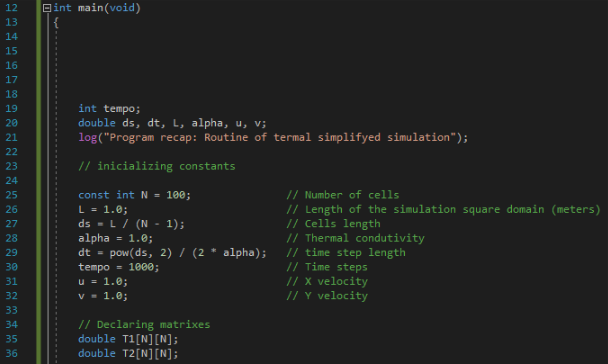
\includegraphics[trim = {0cm 1cm 5cm 1cm}, clip , angle=0, scale=0.65]{images/printCodigo1}
				\caption{Código em c++ no editor.}
			\end{figure}
		\end{minipage}
	\end{frame}
	
	
	
	
	
	\begin{frame}
		\frametitle{OPENGL implementado em C++}
		O OPENGL para c++ é a implementação mais popular da API, junto da implementação em JAVA. Mas ela possui adaptações para várias linguagens, por meio de "bindings", ou seja, ligações do código às funções em c. A API fornece só uma forma de se comunicar com a placa de vídeo presente no computador. Não consiste em uma biblioteca, mas em um conjunto de definições de funções que já vem de fábrica instaladas nas placas de vídeo. Assim a API identifica a placa de vídeo e funciona como uma ponte entre o código e as funcionalidades nativas da placa de vídeo.
		\begin{minipage}[h!]{0.49\textwidth}
			\begin{figure}[h!]
				\centering
				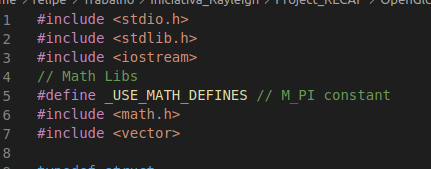
\includegraphics[trim = {0cm 1cm 5cm 1cm}, clip , angle=0, scale=0.35]{images/cmaismaiscode}
				\caption{Chamada das definições OPENGL.}
			\end{figure}
		\end{minipage}
		\begin{minipage}[h!]{0.49\textwidth}
			\begin{figure}[h!]
				\centering
				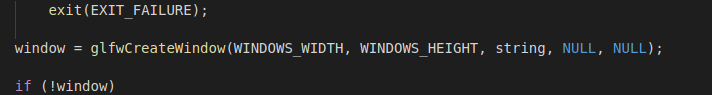
\includegraphics[trim = {0cm 1cm 5cm 1cm}, clip , angle=0, scale=0.35]{images/criandojanela}
				\caption{Criação de janela com a biblioteca GLFW.}
			\end{figure}
			\begin{figure}[h!]
				\centering
				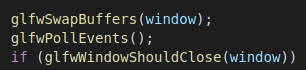
\includegraphics[trim = {0cm 0cm 0cm 0cm}, clip , angle=0, scale=0.35]{images/eventos}
				\caption{Função para processamento de evento GLFW.}
			\end{figure}
		
		\end{minipage}
	\end{frame}

	


	
	\begin{frame}
		\frametitle{Resultados iniciais}
		\begin{minipage}[h!]{0.49\textwidth}
			$\bullet$  Inicialmente, foi tratado somente condução térmica, as velocidades foram setadas em zero, resultando na solução da energia térmica clássica. Com a simulação de alguns casos, obteve-se os resultados ao lado.Apesar de se obedecer aos quesitos de convergência, não se consegue desenvolver uma simulação muito grande. E o resultado parece ser dependente da malha.
		\end{minipage}
		\begin{minipage}[h!]{0.49\textwidth}
			\begin{figure}[h!]
				\centering
				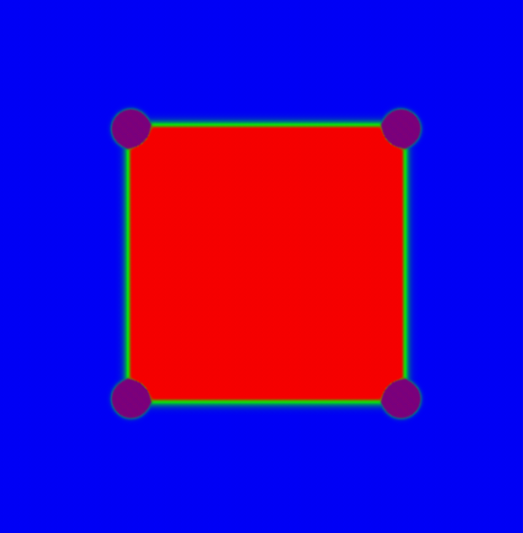
\includegraphics[trim = {1cm 1cm 1cm 1cm}, clip , angle=0, scale=0.45]{images/preliminar_results_1}
				\caption{Divergência da solução.}
			\end{figure}
		\end{minipage}
	\end{frame}





	\begin{frame}
		\frametitle{Resultados iniciais}
		\begin{minipage}[h!]{0.49\textwidth}
			\begin{figure}[h!]
				\centering
				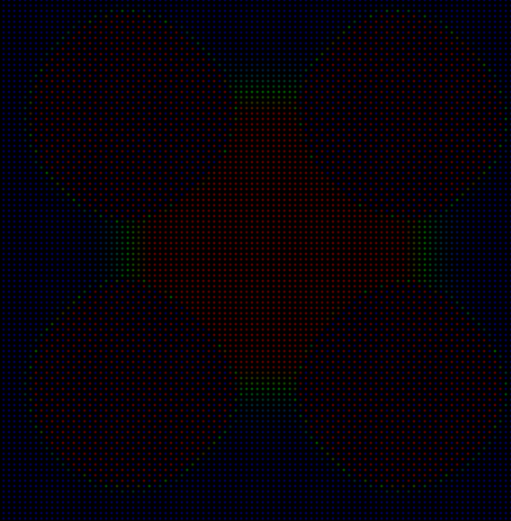
\includegraphics[trim = {1cm 1cm 1cm 1cm}, clip , angle=0, scale=0.38]{images/preliminar_results_2}
				\caption{Simulação com poucos pontos.}
			\end{figure}
		\end{minipage}
		\begin{minipage}[h!]{0.49\textwidth}
			\begin{figure}[h!]
				\centering
				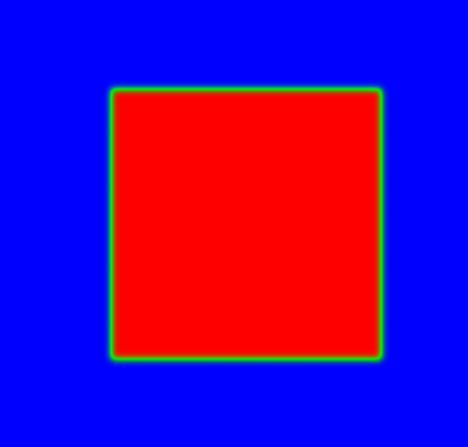
\includegraphics[trim = {1cm 1cm 1cm 1cm}, clip , angle=0, scale=0.45]{images/preliminar_results_3}
				\caption{Simulação com muitos pontos antes da divergência.}
			\end{figure}
		\end{minipage}
	\end{frame}





	\begin{frame}
		\frametitle{Resultados iniciais}
		$\bullet$ Mas, diminuindo-se o passo de tempo a valores muito pequenos, foi possível se alcançar a convergência para longos tempos de simulação, foi então que se observou um erro numérico na determinação do passo de tempo, corrigindo ele, obteve-se:\\
		\begin{minipage}[h!]{0.30\textwidth}
			\begin{figure}[h!]
				\centering
				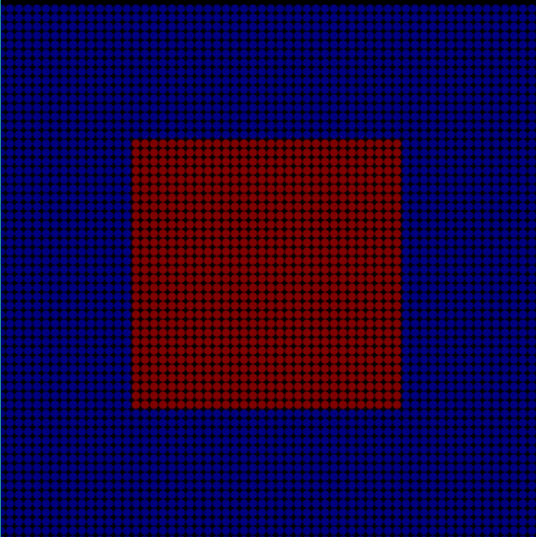
\includegraphics[trim = {1cm 1cm 1cm 1cm}, clip , angle=0, scale=0.3]{images/sucesso_!}
				\caption{Condição inicial.}
			\end{figure}
		\end{minipage}
		\begin{minipage}[h!]{0.30\textwidth}
			\begin{figure}[h!]
				\centering
				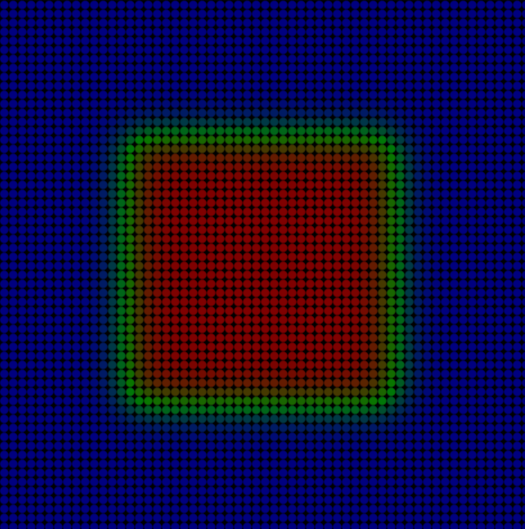
\includegraphics[trim = {1cm 1cm 1cm 1cm}, clip , angle=0, scale=0.3]{images/sucesso_2}
				\caption{Situação intermediária.}
			\end{figure}
		\end{minipage}
		\begin{minipage}[h!]{0.30\textwidth}
			\begin{figure}[h!]
				\centering
				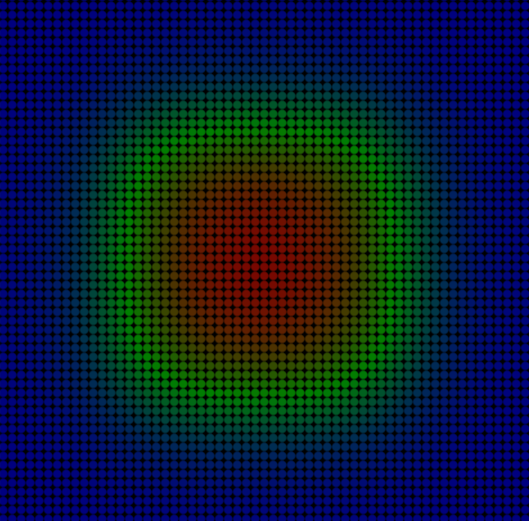
\includegraphics[trim = {1cm 1cm 1cm 1cm}, clip , angle=0, scale=0.3]{images/sucesso_3}
				\caption{Simulação bem sucedida.}
			\end{figure}
		\end{minipage}
	\end{frame}





	\begin{frame}
		\frametitle{Resultados iniciais}
		$\bullet$ Tendo-se sucesso no método clássico, acionou-se a velocidade a 5 m/s obtendo-se o seguinte resultado:\\
		\begin{minipage}[h!]{0.30\textwidth}
			\begin{figure}[h!]
				\centering
				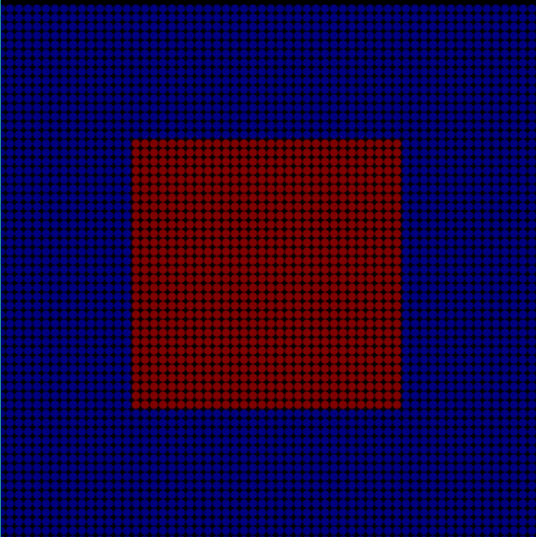
\includegraphics[trim = {1cm 1cm 1cm 1cm}, clip , angle=0, scale=0.3]{images/sucesso_!}
				\caption{Condição inicial.}
			\end{figure}
		\end{minipage}
		\begin{minipage}[h!]{0.30\textwidth}
			\begin{figure}[h!]
				\centering
				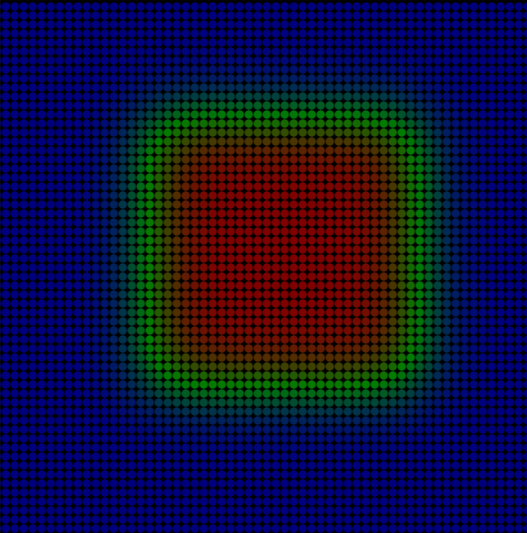
\includegraphics[trim = {1cm 1cm 1cm 1cm}, clip , angle=0, scale=0.3]{images/sucesso_velocidade_2}
				\caption{Situação intermediária.}
			\end{figure}
		\end{minipage}
		\begin{minipage}[h!]{0.30\textwidth}
			\begin{figure}[h!]
				\centering
				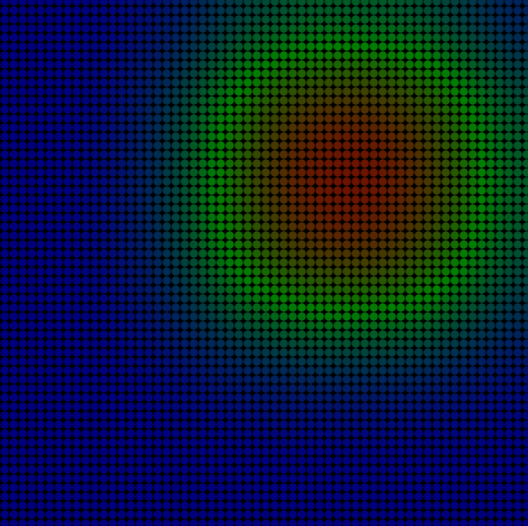
\includegraphics[trim = {1cm 1cm 1cm 1cm}, clip , angle=0, scale=0.3]{images/sucesso_velocidade_3}
				\caption{Simulação bem sucedida.}
			\end{figure}
		\end{minipage}
	\end{frame}	





	\begin{frame}
		\frametitle{Validação e análise de erros e convergência}
		\begin{minipage}[h!]{0.77\textwidth}
			$\bullet$ Com um programa funcional, chegou então a hora de se fazer uma análise de erros a fim de se validar quantitativamente o método. até mesmo com uma análise na ordem de convergência.  \\
			$\bullet$ Para isso, utilizou-se do artifício da solução manufaturada, que consiste em se criar um termo fonte e propor uma solução para T, de forma a se desenvolver uma solução exata para a equação quando acrescida deste termo fonte. Seguem a solução proposta e o termo fonte:
			\begin{equation}
				T = e ^{1 - (x^2 + y^2 + t)}
			\end{equation}
			\begin{equation}
				G = e^{1 - (x^2 + y^2 + t)} \left( 4 \alpha - 2 u x - 2 v y - 4 \alpha (x^2 + y^2) - 1 \right)
			\end{equation}
			$\bullet$ Assim temos a função analítica a ser analisada pelo método numérico como segue:
			\begin{equation}
				\frac{\partial T}{\partial t} + u \frac{\partial T}{\partial x} + v \frac{\partial T}{\partial y} = \alpha \left[  \frac{\partial^2 T}{\partial x^2} + \frac{\partial^2 T}{\partial y^2}   \right] + G 
			\end{equation}
		\end{minipage}
		\begin{minipage}[h!]{0.17\textwidth}
			\begin{figure}[h!]
				\centering
				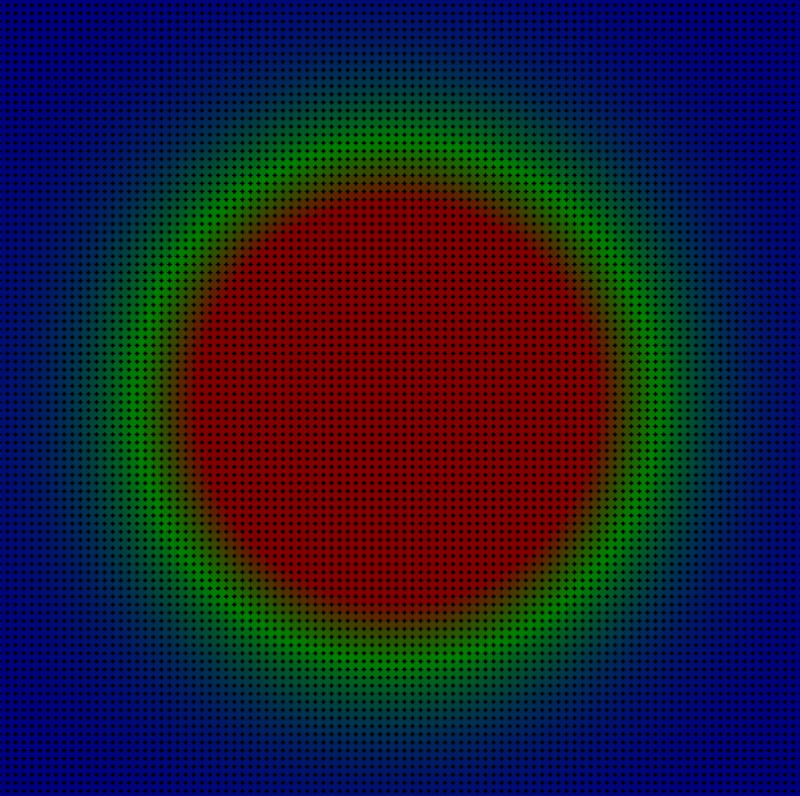
\includegraphics[trim = {0cm 0cm 0cm 0cm}, clip , angle=0, scale=0.1]{images/Analise_manufaturada}
				\caption{Resultado simulado.}
			\end{figure}
			\begin{figure}[h!]
				\centering
				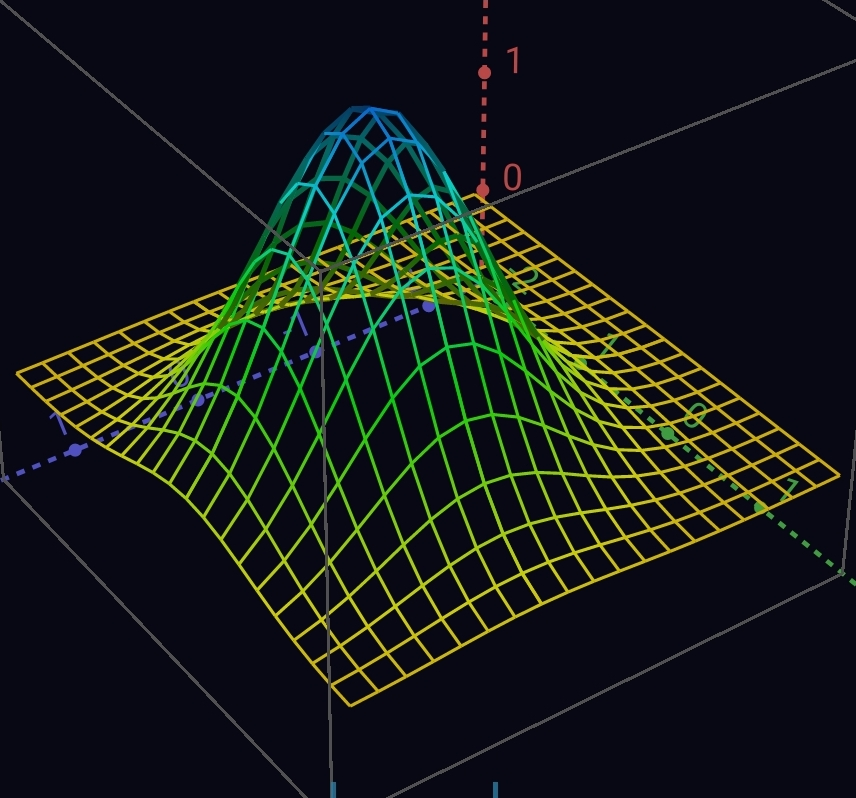
\includegraphics[trim = {0cm 0cm 0cm 0cm}, clip , angle=0, scale=0.07]{images/resultado_analitico}
				\caption{ Resultado exato.}
			\end{figure}
		\end{minipage}
	\end{frame}	





	\begin{frame} 
		\frametitle{Modelo numérico explícito}
		$\bullet$ Com algumas simplificações chega-se na expressão utilizada no código:
		\begin{equation}
			\begin{split}
			T_{i,j}^{k} = T_{i,j}^{k-1} \left( 1 - 4 \frac{\alpha \Delta t}{\Delta s ^2}\right) + T_{i -1, j}^{k-1} \left( \alpha \frac{\Delta t}{\Delta s^2} + u \frac{\Delta t}{2 \Delta s} \right)\\
			+ T_{i,j-1}^{k-1} \left( \alpha \frac{\Delta t}{\Delta s^2} + v \frac{\Delta t}{2 \Delta s} \right) +  T_{i+1,j}^{k-1} \left( \alpha \frac{\Delta t}{ \Delta s^2} - u \frac{\Delta t}{2 \Delta s}\right) \\
			+  T_{i,j+1}^{k-1} \left( \alpha \frac{\Delta t}{\Delta s^2} - v \frac{\Delta t}{2 \Delta s}\right) + G
			\end{split}
		\end{equation}
	\end{frame}





	\begin{frame} 
		\frametitle{Modelo numérico implícito}
		$\bullet$ Com algumas simplificações chega-se na expressão utilizada no código:
		\begin{equation}
			\begin{split}
			T_{i,j}^{k} = \frac{T_{i,j}^{k-1} + T_{i -1, j}^{k} \left( \alpha \frac{\Delta t}{\Delta s^2} + u \frac{\Delta t}{2 \Delta s} \right) 	+ T_{i,j-1}^{k} \left( \alpha \frac{\Delta t}{\Delta s^2} + v \frac{\Delta t}{2 \Delta s} \right)}{ 1 - 4 \frac{\alpha \Delta t}{\Delta s ^2}} \\
			+ \frac{  T_{i+1,j}^{k} \left( \alpha \frac{\Delta t}{ \Delta s^2} - u \frac{\Delta t}{2 \Delta s}\right) 
			+  T_{i,j+1}^{k} \left( \alpha \frac{\Delta t}{\Delta s^2} - v \frac{\Delta t}{2 \Delta s}\right) + G}{ 1 - 4 \frac{\alpha \Delta t}{\Delta s ^2}}
			\end{split}
		\end{equation}
	\end{frame}





	\begin{frame} 
		\frametitle{Resultados das simulações}
		$\bullet$ Dessa forma, foram conduzidas várias simulações em diferentes CFL`s, de forma a se observar o comportamento do erro a partir destes desenvolvimentos, seguem os resultados: \\
		\begin{minipage}[h!]{0.49\textwidth}
			\begin{figure}[h!]
				\centering
				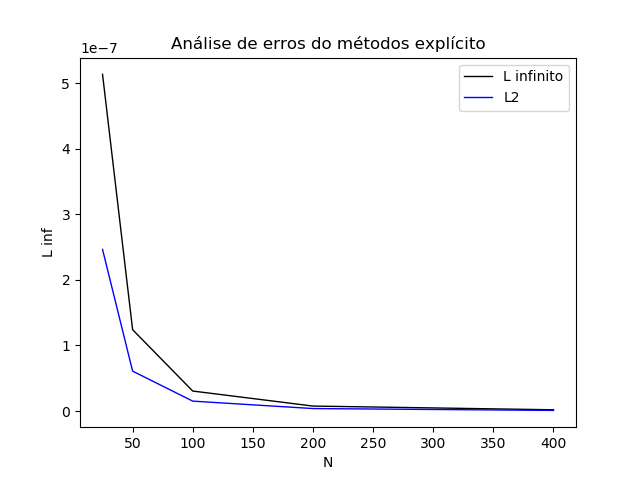
\includegraphics[trim = {0cm 0cm 0cm 0cm}, clip , angle=0, scale=0.4]{images/analise_de_erros_explicito}
				\caption{ Análise de convergência para o método explicito. Uma análise das normas revelou uma convergência de 2 ordem. Quando se dobrava o numero de células, se dividia por aproximadamente 4 o erro.}
			\end{figure}
		\end{minipage}
		\begin{minipage}[h!]{0.49\textwidth}
			\begin{figure}[h!]
				\centering
				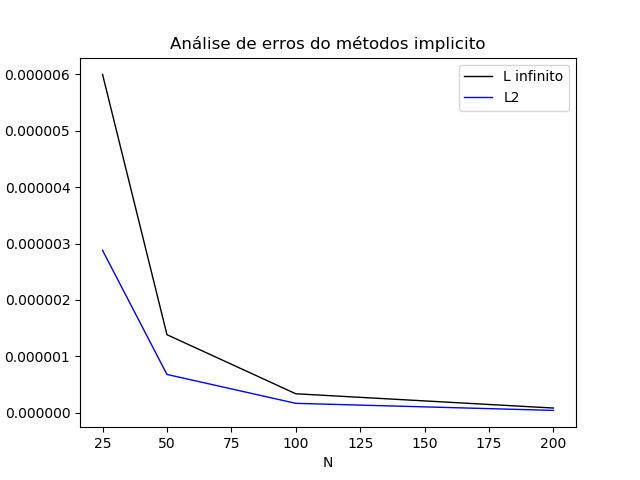
\includegraphics[trim = {0cm 0cm 0cm 0cm}, clip , angle=0, scale=0.4]{images/analise_de_erros_implicito}
				\caption{ Análise de convergência para o método implícito. Uma análise das normas revelou uma convergência de 2 ordem. Quando se dobrava o numero de células, se dividia por aproximadamente 4 o erro.}
			\end{figure}
		\end{minipage}
	\end{frame}





	\begin{frame} 
		\frametitle{Código em FORTRAN}
		\begin{minipage}[h!]{0.49\textwidth}
			
			Diferente do C++, onde se usa a biblioteca GLFW para criação de janelas, no FORTRAN se utiliza o GLUT. Não foi possível localizar bidings para GLFW já prontas. E decidiu-se que seria mais simples aprender a nova biblioteca.
			
			$\bullet$ Foi traduzido do c++ para FORTRAN o código de condução com advecção.\\
			$\bullet$ Casos teste foram utilizados para validação qualitativa.\\
			$\bullet$ Alguns parâmetros de teste notáveis foram: \\
			- Alpha = 97 (Alumínio) \\
			- u = 5 m/s \\
			- v = 5 m/s \\
			$\bullet$ Para o explícito foi obedecida a condição de convergência:
			\begin{equation}
			\Delta t \leq \frac{\Delta s ^2}{4 \alpha} 
			\end{equation}
		\end{minipage}
		\begin{minipage}[h!]{0.49\textwidth}
			\begin{figure}[h!]
				\centering
				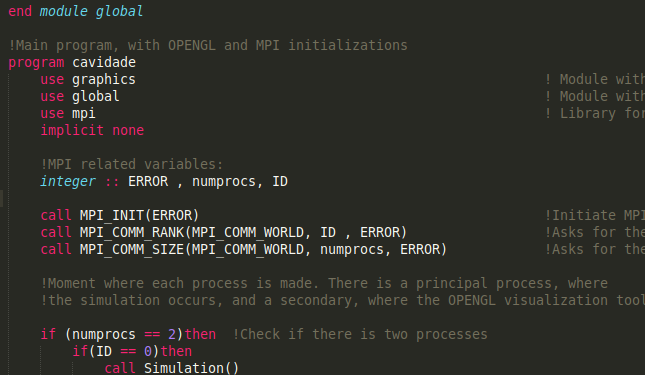
\includegraphics[trim = {0cm 1cm 5cm 1cm}, clip , angle=0, scale=0.45]{images/fortran_code}
				\caption{Código em FORTRAN com implementação de MPI e OPENGL.}
			\end{figure}
		\end{minipage}
	\end{frame}


\tikzstyle{rect} = [draw, rectangle,fill = red!20, text width=6em, text centered, minimum height = 2em ]
\tikzstyle{elli} = [draw, ellipse,fill=white!20,minimum height=2em]
\tikzstyle{circ} = [draw, circle,fill=white!20, minimum width=8pt,inner sep=10pt]
\tikzstyle{diam} = [draw, diamond,fill=white!20,text width=6em, text badly centered, inner sep=0pt]
\tikzstyle{line} = [draw, -latex']


	\begin{frame}
		\frametitle{Uso do MPI no código}
		\begin{minipage}[h!]{0.35\textwidth}
			Criam-se dois processos em paralelo. Um dedicado à renderização dos resultados e o outro dedicado somente à simulação.\\
			A forma encontrada de sincronizar ambos os processos foi dispondo funções de envio e recebimento sempre complementares, garantindo mensagens nos dois sentidos para cada mensagem trocada. 
		\end{minipage}	\hspace{0.5cm}
		\begin{minipage}[h!]{0.59\textwidth}
			\begin{figure}[h]
				\begin{center}
					\begin{tikzpicture}[node distance = 1.5cm, auto]
					\node[rect, rounded corners](step1) {$ Source Code $};
					\node[rect,rounded corners , below of=step1, node distance=2.5cm] (step2) {$ IF(RANK) $};
					\node[rect, right of=step2, node distance=3.5cm] (step3) {$Simulation()$};
					\node[rect, left of=step2, node distance=3.5cm] (step4){$Vizualization()$};
				
					\path[line](step1) -- node [right, text width=4em] {mpirun -n 2.} node [left, text width=4em] {} (step2);
				
					\path[line](step2) -- node [above,near end, text width=4em] { = 0} node (line2) [below, text width=4em] {} (step3);
				
					\path[line](step2) -- node [above,near start, text width=4em] { = 1} node [below, text width=4em] {} (step4);
				
					\end{tikzpicture}
				\end{center}
				\caption{Fluxograma do uso de MPI no algorítmo.}
			\end{figure}
		
		Após a criação dos processos filhos, tem-se a comunicação entre eles por MPI\_SEND e MPI\_RCEV.
		\end{minipage}
	\end{frame}





	\begin{frame}
		\frametitle{Resultados}
	 	Com o devido cuidado com o código foi possível se obter o mesmo resultado do c++ com o fortran:
	 
	 
	\end{frame}












	

%%%%%%%%%%%%%%%%%%%%%%%%%%%%%%%%%%%%%%%%%%%%%%%%%%%%%%%%%%%%%%%%%%%%%%%%%%%%%%%%%%%%%%%%%%%%%%
\section{Modelo físico}

	\begin{frame}
		\frametitle{Hipóteses e considerações sobre o sistema}
		\begin{tabular}{c c}
			{
				\begin{minipage}{0.4\textwidth}
					\small
					\centering
					O problema fluidodinâmico escolhido foi o da cavidade. Ele consiste em uma quantidade de fluido confinada a um sistema termodinâmico com duas fontes de energia térmica como observado na Fig.\ref{sistema_termico_1}.
					
					\vspace{0.2cm}
					
					\flushleft
					As considerações feitas foram:\\
					\quad $\bullet$ O fluido é incompressível e newtoniano, sendo que sua massa específica varia somente em função da temperatura.\\
					\quad $\bullet$ O sistema foi considerado auto-similar na coordenada $z$. \\
					\quad $\bullet$ As superfícies perpendiculares ao eixo $y$ são isoladas termicamente.\\
					\quad $\bullet$ Considera-se uma fonte fria e uma fonte quente nas superfícies perpendiculares ao eixo $x$.\\
				\end{minipage}
			}&{
				\begin{minipage}{0.5\textwidth}
					\begin{figure}
						\centering
						\includegraphics[page = 1,trim={6.0cm 2.0cm 6.0cm 1.5cm},clip=true, scale = 0.4]{images/Cavidade_fisico_1.pdf}
						\caption{Sistema físico da cavidade.}
						\label{sistema_termico_1}
					\end{figure}
				\end{minipage}
			}
		\end{tabular}
	
	\end{frame}





%%%%%%%%%%%%%%%%%%%%%%%%%%%%%%%%%%%%%%%%%%%%%%%%%%%%%%%%%%%%%%%%%%%%%%%%%%%%%%%%%%%%%%%%%%%%%%
\section{Desenvolvimento matemático}

	\begin{frame}
		\frametitle{Equações representativas}
		\flushleft
		Para este desenvolvimento matemático serão utilizadas:\\
		\quad $\bullet$ As equações de Navier Stokes.\\
		\quad $\bullet$ A equação da continuidade.\\
		\quad $\bullet$ A equação de balanço da energia térmica.\\
		\quad $\bullet$ Uma equação de estado.\\
		
		\begin{equation}
		\nabla . \vec{V} = 0
		\end{equation}
		\begin{equation}
		\frac{\partial \vec{V}}{\partial t} +  \vec{V} . {\nabla} \vec{V}  =  -\frac{1}{\rho_o} {\nabla}P + \frac{\rho - \rho_o}{\rho_o} \vec{g} + \nu \nabla ^2 \vec{V}
		\end{equation}
		\begin{equation}
		\frac{\partial T}{\partial t} + \vec{\nabla} . \left( \vec{V}T \right) = \alpha \nabla^2T
		\end{equation}
		\begin{equation}
		\frac{\rho - \rho_o}{\rho_o} = \beta \left( T - T_o\right)
		\end{equation}
	
	\end{frame}




	
	\begin{frame}
		\frametitle{Desenvolvendo pressão e velocidade}
		\flushleft
		Primeiramente se desenvolvem as equações de Navier-Stokes de duas formas:\vspace{0.5cm}
		\centering
		\underline{A partir do domínio da pressão no passo posterior:}
		\begin{equation}
		\frac{\vec{V}^{n + 1} - \vec{V}^{n}}{\Delta t} + \vec{V}^{n} . {\nabla} \vec{V}^{n} = - \frac{1}{\rho_o}\nabla P^{n + 1} + \left( \frac{\rho - \rho_o}{\rho_o} \right) \vec{g} + \nu \nabla^2 \vec{V}^{n}
		\end{equation}\label{equation1}
		\underline{A partir do domínio da pressão no passo atual:}
		\begin{equation}
		\frac{\vec{V}^{\ast{n + 1}} - \vec{V}^{n}}{\Delta t} + \vec{V}^{n} . {\nabla} \vec{V}^{n} = - \frac{1}{\rho_o}\nabla P^{n} + \left( \frac{\rho - \rho_o}{\rho_o} \right) \vec{g} + \nu \nabla^2 \vec{V}^{n}
		\end{equation}
		
		Assim, subtraindo-se as duas, tem-se uma relação que descreve a relação entre os valores do domínio da pressão:
		
		\begin{equation}
		\frac{\vec{V}^{{n + 1}} - \vec{V}^{{\ast n+1} }}{\Delta t} = - \frac{1}{\rho_o}\nabla \left( P^{n+1} - P ^n\right)
		\end{equation}
		
		
		
	\end{frame}




	\begin{frame}
		\frametitle{Diferença de pressão}
		\flushleft
		Assim, descreve-se uma nova variável $ P^\prime $ que denota a diferença na pressão entre os passos, como:
		
		\begin{equation}
		P^\prime = P^{n + 1} - P^n
		\end{equation}
		Assim temos:
		
		\begin{equation}
		\vec{V}^{n+1} - \vec{V}^{\ast{n + 1}} = - \frac{\Delta t}{\rho_o} \nabla P^\prime
		\end{equation}
		
		Aplicando-se o divergente em ambos os lados temos:
		
		\begin{equation}
		\nabla . \vec{V}^{n+1} - \nabla .\vec{V}^{\ast{n + 1}} = - \frac{\Delta t}{\rho_o} \nabla^2 P^\prime
		\end{equation}
		
		A partir da equação da continuidade temos:
		
		\begin{equation}
		\nabla .\vec{V}^{\ast{n + 1}} = \frac{\Delta t}{\rho_o} \nabla^2 P^\prime
		\end{equation}
		
	
	\end{frame}


\tikzstyle{rect} = [draw, rectangle,fill = red!20, text width=5em, text centered, minimum height = 2em ]
\tikzstyle{elli} = [draw, ellipse,fill=white!20,minimum height=2em]
\tikzstyle{circ} = [draw, circle,fill=white!20, minimum width=8pt,inner sep=10pt]
\tikzstyle{diam} = [draw, diamond,fill=white!20,text width=6em, text badly centered, inner sep=0pt]
\tikzstyle{line} = [draw, -latex']

	\begin{frame}
		\frametitle{Fluxograma de dados por iteração}
		\flushleft
		Assim tem-se um valor inicial de velocidade estimada, que é utilizado para corrigir o domínio de pressão.
		\begin{figure}[h]
			\begin{center}
				\begin{tikzpicture}[node distance = 1.5cm, auto]
					\node[rect, rounded corners](step1) {$\vec{V}^n $};
					\node[rect,rounded corners , right of=step1, node distance=4.5cm] (step2) {$\vec{V}^{* n + 1} $};
					\node[rect, right of=step2, node distance=4.5cm] (step3) {$P^\prime$};
					\node[rect, right of=step3, node distance=4.5cm] (step4){$P^{n + 1}$};
					\node[rect, rounded corners, below of=step4, node distance=2.5cm](step5){$ \vec{V}^{n+1}$};
					
					\path[line](step1) -- node [above, text width=4em] {Resolução explicita.} node [below, text width=4em] {Eq.5} (step2);
					
					\path[line](step2) -- node [above, text width=4em] {Resolução implicita.} node (line2) [below, text width=4em] {Eq.11} (step3);
					
					\path[line](step3) -- node [above, text width=4em] {Resolução explícita.} node [below, text width=4em] {Eq.8} (step4);
					
					\path[line](step4) -- node [left, text width=5em] {Resolução explicita. Eq.9} (step5);
					
					\path[line](step5) -| node [right, near end, text width=6em] {Mais tempo na correção de pressão.} (line2);
					
					\path[line](step5) -| node [right, near end, text width=6em] {Atualiza\\domínio.} node [below, near start, text width=12em] {Checa continuidade.} (step1);
				\end{tikzpicture}
			\end{center}
		\caption{Fluxograma do loop principal do algoritmo.}
		\end{figure}
	\end{frame}
	
	
	
	
	
	\begin{frame}
		\frametitle{Desenvolvimento das equações de Navier-Stokes}
		\centering
		\begin{equation}
			\frac{\partial \vec{V}}{\partial t} +  \vec{V} . {\nabla} \vec{V}  =  -\frac{1}{\rho_o} {\nabla}P + \frac{\rho - \rho_o}{\rho_o} \vec{g} + \nu \nabla ^2 \vec{V}
		\end{equation}
		Com as equações de Navier-Stokes no formato vetorial, separam-se nas três componentes:
		
		\begin{equation}
			\frac{\partial u}{\partial t} + u\frac{\partial u}{\partial x} + v\frac{\partial u}{\partial y} + w\frac{\partial u }{\partial z}  =  -\frac{1}{\rho_o} \frac{\partial P}{\partial x} + \frac{\rho - \rho_o}{\rho_o} g_x + \nu \left( \frac{\partial ^2 u}{\partial x^2} + \frac{\partial ^2 u}{\partial y^2} + \frac{\partial ^2 u}{\partial z^2} \right)
		\end{equation}
		
		\begin{equation}
			\frac{\partial v}{\partial t} + u\frac{\partial v}{\partial x} + v\frac{\partial v}{\partial y} + w\frac{\partial v }{\partial z}  =  -\frac{1}{\rho_o} \frac{\partial P}{\partial y} + \frac{\rho - \rho_o}{\rho_o} g_y + \nu \left( \frac{\partial ^2 v}{\partial x^2} + \frac{\partial ^2 v}{\partial y^2} + \frac{\partial ^2 v}{\partial z^2} \right)
		\end{equation}
	
		\begin{equation}
			\frac{\partial w}{\partial t} + u\frac{\partial w}{\partial x} + v\frac{\partial w}{\partial y} + w\frac{\partial w }{\partial z}  =  -\frac{1}{\rho_o} \frac{\partial P}{\partial z} + \frac{\rho - \rho_o}{\rho_o} g_z + \nu \left( \frac{\partial ^2 w}{\partial x^2} + \frac{\partial ^2 w}{\partial y^2} + \frac{\partial ^2 w}{\partial z^2} \right)
		\end{equation}
	\end{frame}





	\begin{frame}
		\frametitle{Desenvolvimento das equações de Navier-Stokes}
		\centering
		\begin{equation}
			\frac{\partial u}{\partial t} + u\frac{\partial u}{\partial x} + v\frac{\partial u}{\partial y} + {\color{red} w\frac{\partial u }{\partial z} } =  -\frac{1}{\rho_o} \frac{\partial P}{\partial x} + \frac{\rho - \rho_o}{\rho_o} g_x + \nu \left( \frac{\partial ^2 u}{\partial x^2} + \frac{\partial ^2 u}{\partial y^2} + { \color{red} \frac{\partial ^2 u}{\partial z^2} } \right)
		\end{equation}
	
		\begin{equation}
			\frac{\partial v}{\partial t} + u\frac{\partial v}{\partial x} + v\frac{\partial v}{\partial y} + {\color{red} w\frac{\partial v }{\partial z} } =  -\frac{1}{\rho_o} \frac{\partial P}{\partial y} + \frac{\rho - \rho_o}{\rho_o} g_y + \nu \left( \frac{\partial ^2 v}{\partial x^2} + \frac{\partial ^2 v}{\partial y^2} + { \color{red} \frac{\partial ^2 v}{\partial z^2} } \right)
		\end{equation}
		
		{\color{red}
			\begin{equation}
				\frac{\partial w}{\partial t} + u\frac{\partial w}{\partial x} + v\frac{\partial w}{\partial y} + w\frac{\partial w }{\partial z}  =  -\frac{1}{\rho_o} \frac{\partial P}{\partial z} + \frac{\rho - \rho_o}{\rho_o} g_z + \nu \left( \frac{\partial ^2 w}{\partial x^2} + \frac{\partial ^2 w}{\partial y^2} + \frac{\partial ^2 w}{\partial z^2} \right)
			\end{equation}
		}
		
		Tirando os termos referentes à dimensão z, a partir de considerações de autosimilaridade.
		
		
	\end{frame}




	
	\begin{frame}
		\frametitle{Desenvolvimento das equações de Navier-Stokes}
		\centering
		\begin{equation}
			\frac{\partial u}{\partial t} + u\frac{\partial u}{\partial x} + v\frac{\partial u}{\partial y} =  -\frac{1}{\rho_o} \frac{\partial P}{\partial x} + \frac{\rho - 	\rho_o}{\rho_o} g_x + \nu \left( \frac{\partial ^2 u}{\partial x^2} + \frac{\partial ^2 u}{\partial y^2} \right)
		\end{equation}
	
		\begin{equation}
			\frac{\partial v}{\partial t} + u\frac{\partial v}{\partial x} + v\frac{\partial v}{\partial y} =  -\frac{1}{\rho_o} \frac{\partial P}{\partial y} + \frac{\rho - \rho_o}{\rho_o} g_y + \nu \left( \frac{\partial ^2 v}{\partial x^2} + \frac{\partial ^2 v}{\partial y^2} \right)
		\end{equation}
		Discretizando estes termos, a partir de expansões em série de Taylor, tem-se:
		\begin{equation}
			\begin{split}
			\frac{u_{i , j}^{\ast k + 1} - u_{i , j}^{k}}{\Delta t} + u_{i , j}^{k}\frac{u_{i + 1 , j}^k - u_{i - 1 , j}^k  }{2 \Delta x} + v_{i , j}^{k}\frac{u_{i , j+ 1}^k - u_{i, j-1}^k  }{2 \Delta y} =  -\frac{1}{\rho_o} \frac{P_{i, j}^k - P_{i - 1, j}^k}{\Delta x} \\ + \frac{\rho - 	\rho_o}{\rho_o} g_x + \nu \left( \frac{u_{i+1 , j}^k - 2 u_{i,j}^k + u_{i-1,j}^k}{\Delta x^2} + \frac{u_{i , j+1}^k - 2 u_{i,j}^k + u_{i,j-1}^k}{\Delta y^2} \right)
			\end{split}
		\end{equation}
		
	
	\end{frame}




	\begin{frame}
		\frametitle{Desenvolvimento das equações de Navier-Stokes}
		Dessa forma tem-se as duas equações de transporte de momento discretizadas:
		\begin{equation}
			\begin{split}
			\frac{u_{i , j}^{\ast k + 1} - u_{i , j}^{k}}{\Delta t} + u_{i , j}^{k}\frac{u_{i + 1 , j}^k - u_{i - 1 , j}^k  }{2 \Delta x} + v_{i , j}^{k}\frac{u_{i , j+ 1}^k - u_{i, j-1}^k  }{2 \Delta y} =  -\frac{1}{\rho_o} \frac{P_{i, j}^k - P_{i - 1 , j}^k}{\Delta x} \\ + \frac{\rho - 	\rho_o}{\rho_o} g_x + \nu \left( \frac{u_{i+1 , j}^k - 2 u_{i,j}^k + u_{i-1,j}^k}{\Delta x^2} + \frac{u_{i , j+1}^k - 2 u_{i,j}^k + u_{i,j-1}^k}{\Delta y^2} \right)
			\end{split}
		\end{equation}
		\begin{equation}
			\begin{split}
			\frac{v_{i , j}^{\ast k + 1} - v_{i , j}^{k}}{\Delta t} + u_{i , j}^{k}\frac{v_{i + 1 , j}^k - v_{i - 1 , j}^k  }{2 \Delta x} + v_{i , j}^{k}\frac{v_{i , j+ 1}^k - v_{i, j-1}^k  }{2 \Delta y} =  -\frac{1}{\rho_o} \frac{P_{i , j}^k - P_{i , j - 1}^k}{\Delta y} \\ + \frac{\rho - 	\rho_o}{\rho_o} g_x + \nu \left( \frac{v_{i+1 , j}^k - 2 v_{i,j}^k + v_{i-1,j}^k}{\Delta x^2} + \frac{v_{i , j+1}^k - 2 v_{i,j}^k + v_{i,j-1}^k}{\Delta y^2} \right)
			\end{split}
		\end{equation}
	\end{frame}




	\begin{frame}
		\frametitle{Efetuando a correção na pressão}
		Resgatando a equação para correção da pressão, tem-se:
		\begin{equation}
			\nabla .\vec{V}^{\ast{n + 1}} = \frac{\Delta t}{\rho_o} \nabla^2 P^\prime
		\end{equation}
		Discretizando a equação:
		\begin{equation}
			\frac{u_{i + 1 , j}^{\ast k + 1} - u_{i , j}^{\ast k + 1}}{\Delta x} + \frac{v_{i , j + 1}^{\ast k + 1} - v_{i , j}^{\ast k + 1}}{\Delta y} = \frac{\Delta t}{\rho_o} * \left( \frac{\partial^2 P^\prime}{\partial x^2} + \frac{\partial^2 P^\prime}{\partial y^2}\right) 
		\end{equation}
		
	\end{frame}



%%%%%%%%%%%%%%%%%%%%%%%%%%%%%%%%%%%%%%%%%%%%%%%%%%%%%%%%%%%%%%%%%%%%%%%%%%%%%%%%%%%%%%%%%%%%%%	
\section{Agradecimentos}
			
	\begin{frame}	
		\begin{center}
		Obrigado às entidades cujo auxílio fora inestimável ao andamento deste trabalho. 
		\end{center}
		\placelogomflab 
		\frametitle{Agradecimentos}
		\begin{center}
		\begin{tabular}{c c}
			{
				
\includegraphics[trim=0.0cm 0.0cm 0.0cm 0.0cm,clip=true,height=0.2\textheight]{figuras_presentation_template/petrobras.png}
			}&{
				
\includegraphics[trim=0.0cm 0.0cm 0.0cm 0.0cm,clip=true,height=0.2\textheight]{figuras_presentation_template/logo_mflab.png}}\\
				{
\includegraphics[trim=0.0cm 0.0cm 0.0cm 0.0cm,clip=true,height=0.2\textheight]{figuras_presentation_template/cnpq.png}
			}&{
				
\includegraphics[trim=0.0cm 0.0cm 0.0cm 0.0cm,clip=true,height=0.2\textheight]{figuras_presentation_template/CAPES.png}}\\
				{
\includegraphics[trim=0.0cm 0.0cm 0.0cm 0.0cm,clip=true,height=0.2\textheight]{figuras_presentation_template/FAPEMIG.jpg}
			}&{
				
\includegraphics[trim=0.0cm 0.0cm 0.0cm 0.0cm,clip=true,height=0.2\textheight]{figuras_presentation_template/UFU_black.jpg}
			}
		\end{tabular}
		\end{center}
			
	\end{frame}
		
			
		
		
		
\end{document}




		



%%%%%%%%%%%%%%%%%%%%%%%%%%%%%%%%%%%%%%% Exemplo de formatação de imagens		
%		\begin{frame}
%			\frametitle{Adição de fronteiras extras}
%			\begin{tabular}{c c}
%				
%				{\includegraphics[trim=0.0cm 0.0cm 0.0cm 0.0cm,clip=true,loop,height=0.5\textheight]{figuras/filtration_depois.png}}&{\includegraphics[trim=0.0cm 0.0cm 0.0cm 0.0cm,clip=true,loop,height=0.4\textheight]{figuras/filtration_depois_zoom.png}}\\
%				
%			\end{tabular}
%			
%		\end{frame}




%%%%%%%%%%%%%%%%%%%%%%%%%%%%%%%%%%%%%% Exemplo de formatação de imagens		
%		\begin{frame}
%			\frametitle{Agora}
%			\centering
%			\begin{tabular}{c}
%				
%				{\includegraphics[trim=0.00cm 2.0cm 0.0cm 2.0cm,clip=true,loop,width=0.9\textwidth]{figuras/t_x_51f.png}}\\{\includegraphics[trim=0.01cm 0.0cm 0.01cm 0.0cm,clip=true,loop,width=0.9\textwidth]{figuras/t_x_51999.png}}\\{\includegraphics[trim=0.01cm 0.0cm 0.01cm 0.0cm,clip=true,loop,width=0.9\textwidth]{figuras/t_x_51999g.png}}\\{\includegraphics[trim=0.01cm 0.0cm 0.01cm 0.0cm,clip=true,loop,width=0.9\textwidth]{figuras/t_x_51999y.png}}\\{\includegraphics[trim=0.01cm 0.0cm 0.01cm 0.0cm,clip=true,loop,width=0.9\textwidth]{figuras/t_x_51999b.png}}
%				
%			\end{tabular}
%			
%		\end{frame}





%%%%%%%%%%%%%%%%%%%%%%%%%%%%%%%%%%%%%  Formatação de equações:		
%		\begin{frame}
%			\frametitle{Newton-Raphson}
%			
%			\flushleft
%			Método de interface com jacobiano composto:
%			
%			\centering
%			\begin{equation}\label{forte_eqNewton}
%			K(D+\Delta D) \approx K(D)+\Delta D \, J(D)
%			\end{equation}
%			\begin{equation}\label{forte_eqNewton2}
%			K(D) =  Estrutura(Fluido(D))-D =  0
%			\end{equation}
%			\begin{equation}\label{forte_eqNewton3}
%			J(D) =  Estrutura'(Fluido(D)) \, Fluido'(D)-I
%			\end{equation}
%			\begin{equation}\label{forte_eqNewton4}
%			Fluido(D): \mathbb{R}^{n} \to \mathbb{R}^{m}
%			\end{equation}
%			
%			\flushleft
%			$Fluido'(D)$ é de tamanho $m x n$
%			
%			\centering
%			
%			\begin{equation}\label{forte_eqNewton5}
%			Estrutura(F): \mathbb{R}^{m} \to \mathbb{R}^{n}
%			\end{equation}
%			
%			\flushleft
%			$Estrutura'(F)$ é de tamanho $n x m$\\
%			$Estrutura'(Fluido(D)) \, Fluido'(D)$ e $I$ é de tamanho $n x n$
%		\end{frame}




%%%%%%%%%%%%%%%%%%%%%%%%%%%%%%%%%%%%%%%%%%% Vários exemplos de formatação textual:		


%		\begin{frame}
%			\frametitle{Conveniência do método de Multi Direct Forcing}
%			
%			\flushleft
%			\textbf{Fraco:}\\
%			$\bullet$ Predição da velocidade.\\
%			$\bullet$ MDF. (Imposição da condição de dirichlet na interface e cálculo da força)\\
%			$\bullet$ Estrutura.\\
%			$\bullet$ Poisson.\\
%			$\bullet$ Correção de velocidade e pressão.\\ \\
%
%			\textbf{Forte:}\\
%			$\bullet$ Predição da velocidade.\\
%			while \\
%			\quad	$\longrightarrow$ MDF.\\
%			\quad	$\longrightarrow$ Estrutura.\\
%			end\\
%			$\bullet$ Poisson.\\
%			$\bullet$ Correção de velocidade e pressão.\\
%
%		\end{frame}

		

%		
%%%%%%%%%%%%%%%%%%%%%%%%%%%%%%%%%  Modelo duas fotos lado a lado:


%		\begin{frame}
%		\frametitle{Limite do fraco}
%			ct=121
%			mi=200
%			\begin{tabular}{c c}
%			{\includegraphics[width=0.45\linewidth]{../../simulacoes_Estudo_dirigido2/fraco_mi_200_0_15_ct141/figuras/estrutura/vel_151}}&
%		   {\includegraphics[width=0.45\linewidth]{../../simulacoes_Estudo_dirigido2/fraco_mi_200_0_15_ct141/figuras/estrutura/vel_251}}\\
%		   {(a) Velocidade em linha centro da estrutura} & {(b) Velocidade transversal centro da estrutura}
%		\end{tabular}
%		\end{frame}



%%%%%%%%%%%%%%%%%%%%%%%%%%%%%%%%%%  Modelo tabela :

%		\begin{frame}
%			\frametitle{Comparação número de iterações}
%			\begin{tabular}{c c c c}
%				\hline
%				Método & Mínimo     &    Máximo &  Média\\ \hline
%				FPI MDF variável & 8     &    101 &  8.9764764764764760\\
%				FPI MDF fixo & 8     &     11 &  8.9099099099099099\\
%				QN Primeiro método de Broyden MDF variável & 18    &     101 &  18.281281281281281 \\ \hline
%			\end{tabular}
%		\end{frame}	




